\documentclass{article}
\usepackage{graphicx}
\usepackage{fancyhdr}
\usepackage{float}
\usepackage{lipsum} % For dummy text

% Configuration du package fancyhdr
\pagestyle{fancy}
\fancyhf{}
\fancyhead[L]{Università di Corsica} % Section title on the left
\fancyhead[C]{TD2} % Centered title
\fancyhead[R]{SANNA Thomas} % Page number on the right
\fancyfoot[L]{SANNA Thomas} % Author on the left
\fancyfoot[C]{Page n°\thepage} % Page number in the center
\fancyfoot[R]{\today} % Date on the right

\begin{document}

\title{Conception Orientée Objet - TD2}
\author{SANNA Thomas}
\date{\today}

\maketitle

\section*{Exercice 2}

\subsection{Classe générale "Bâtiment"}

\begin{figure}[H]
  \centering
  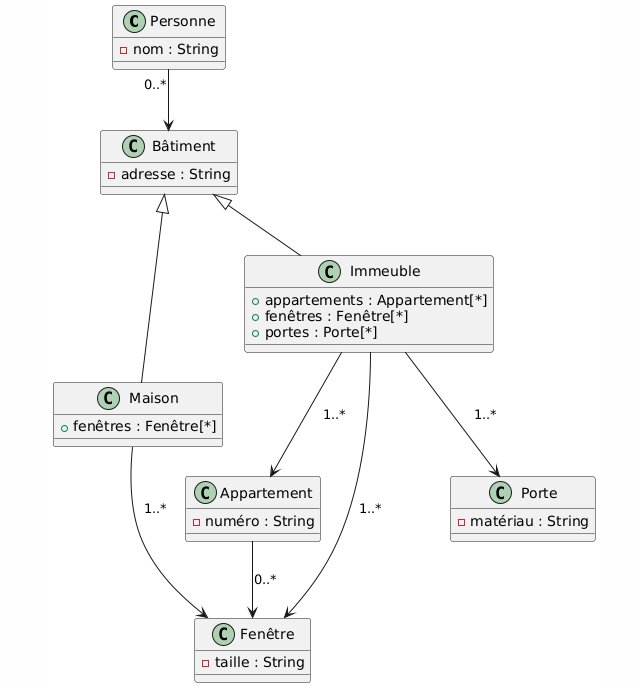
\includegraphics[width=\textwidth]{exo2-1.png}
  \caption{Diagramme de classes pour l'exercice 2}
\end{figure}

\subsection{Structure spécifique pour Maison et Immeuble}

\begin{figure}[H]
  \centering
  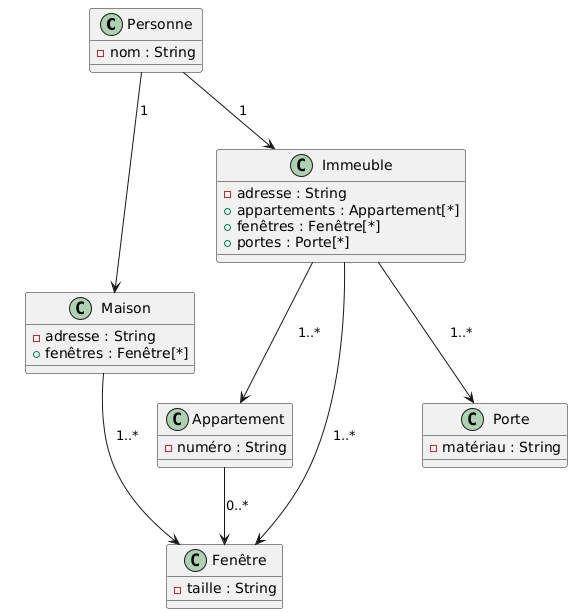
\includegraphics[width=\textwidth]{exo2-2.png}
  \caption{Diagramme de classes pour l'exercice 2 (suite)}
\end{figure}

\section*{Exercice 3}

\subsection*{Présentation des Classes et Associations}

\subsubsection*{1. Identification des classes}

Voici les classes principales à extraire du texte :

\begin{itemize}
  \item \textbf{Vol} : Représente le vol avec ses informations générales.
  \item \textbf{Départ} : Représente un vol programmé à une date donnée avec des informations associées.
  \item \textbf{Passager} : Représente une personne enregistrée pour un départ.
  \item \textbf{Avion} : Représente l’avion affecté à un départ.
  \item \textbf{Personnel} : Représente un employé de la compagnie aérienne.
  \begin{itemize}
    \item \textbf{PersonnelNavigant} (héritant de Personnel) : Représente le personnel qui travaille à bord du vol.
    \begin{itemize}
      \item \textbf{Pilote} (héritant de PersonnelNavigant) : Représente les pilotes.
      \item \textbf{Hôtesse/Stewart} (héritant de PersonnelNavigant) : Représente les hôtesses et stewards.
    \end{itemize}
    \item \textbf{PersonnelNonNavigant} (héritant de Personnel) : Représente le personnel non navigant.
  \end{itemize}
\end{itemize}

\subsubsection*{2. Identification des associations entre classes}

\begin{itemize}
  \item \textbf{Vol - Départ} : Un vol peut avoir plusieurs départs, mais un départ est lié à un seul vol.
  \item \textbf{Départ - Passager} : Un départ peut avoir plusieurs passagers, et un passager peut être enregistré pour plusieurs départs.
  \item \textbf{Départ - Avion} : Un avion est affecté à un départ, un avion peut être utilisé pour plusieurs départs.
  \item \textbf{Départ - PersonnelNavigant/PersonnelNonNavigant} : Plusieurs membres du personnel (navigants et non navigants) sont affectés à chaque départ.
  \item \textbf{Pilote/PersonnelNavigant - Départ} : Un ou deux pilotes et entre 2 et 10 hôtesses/stewards sont affectés à chaque départ.
\end{itemize}

\subsubsection*{3. Position des attributs dans les classes}

\begin{itemize}
  \item \textbf{Vol}
  \begin{itemize}
    \item Numéro de vol
    \item Ville de départ
    \item Ville d’arrivée
    \item Heure de départ
    \item Durée
    \item Jour de la semaine
  \end{itemize}
  \item \textbf{Départ}
  \begin{itemize}
    \item Date du départ
    \item Quantité de carburant utilisée (en fonction de la date)
  \end{itemize}
  \item \textbf{Avion}
  \begin{itemize}
    \item Numéro
    \item Type
    \item Capacité
  \end{itemize}
  \item \textbf{Personne}
  \begin{itemize}
    \item Nom
    \item Adresse
    \item Numéro de téléphone
  \end{itemize}
  \item \textbf{Passager} : Pas d’attribut spécifique (hérite de Personne)
  \item \textbf{Personnel} : Pas d’attribut spécifique (hérite de Personne)
  \item \textbf{PersonnelNavigant}
  \begin{itemize}
    \item Nombre d’heures de vol
  \end{itemize}
  \item \textbf{Pilote} : Pas d’attribut spécifique (hérite de PersonnelNavigant)
  \item \textbf{Hôtesse/Stewart} : Pas d’attribut spécifique (hérite de PersonnelNavigant)
  \item \textbf{PersonnelNonNavigant} : Pas d’attribut spécifique (hérite de Personnel)
\end{itemize}

\subsubsection*{4. Identification des généralisations}

\begin{itemize}
  \item \textbf{Personne} est une classe abstraite.
  \item \textbf{Personnel} et \textbf{Passager} sont des spécialisations de \textbf{Personne}.
  \item \textbf{PersonnelNavigant} et \textbf{PersonnelNonNavigant} sont des spécialisations de \textbf{Personnel}.
  \item \textbf{Pilote} et \textbf{Hôtesse/Stewart} sont des spécialisations de \textbf{PersonnelNavigant}.
\end{itemize}

\begin{figure}[H]
  \centering
  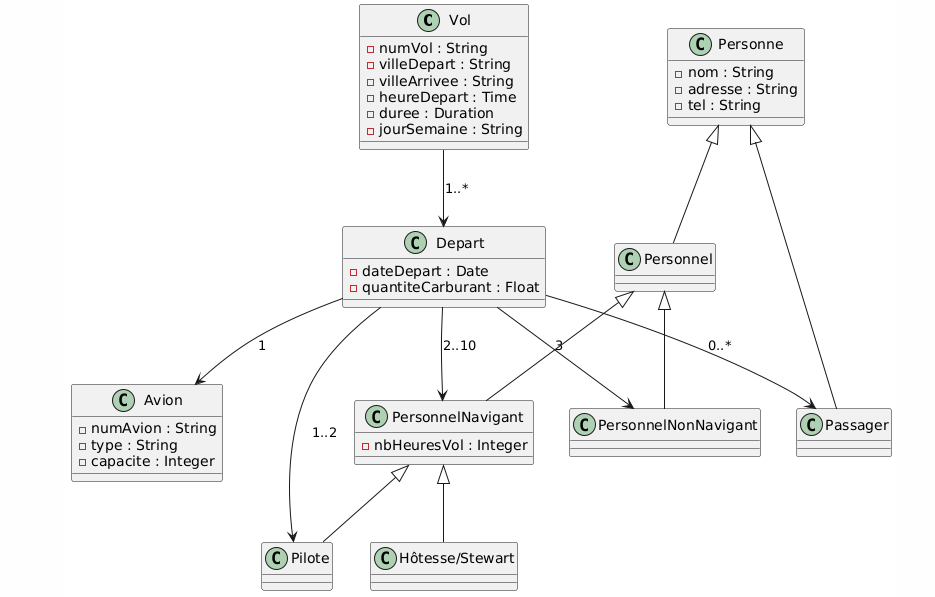
\includegraphics[width=\textwidth]{exo3.png}
  \caption{Diagramme de classes pour l'exercice 3}
\end{figure}

\section*{Exercice 4}

\subsection*{Modélisation des Classes pour une Université}

\subsubsection*{1. Identification des Classes}

Les classes principales à modéliser dans ce contexte sont :

\begin{itemize}
  \item \textbf{Université} : L'entité qui propose les diplômes et gère les inscriptions.
  \item \textbf{Diplôme} : Représente un diplôme, qui est composé de plusieurs unités d'enseignement (UE).
  \item \textbf{UE (Unité d'Enseignement)} : Représente une unité d'enseignement obligatoire ou optionnelle.
  \item \textbf{Étudiant} : Représente un étudiant qui s'inscrit à des diplômes et à des UE.
  \item \textbf{Dossier} : Représente le dossier universitaire d'un étudiant, contenant ses informations personnelles et académiques.
  \item \textbf{InscriptionDiplôme} : Représente l'inscription d'un étudiant à un diplôme, avec le choix des UE optionnelles.
  \item \textbf{InscriptionUE} : Représente l'inscription d'un étudiant à une UE spécifique.
  \item \textbf{Scolarité} : Le service qui gère les inscriptions et l’édition des listes.
\end{itemize}

\subsubsection*{2. Identification des Associations entre Classes}

\begin{itemize}
  \item \textbf{Université - Diplôme} : L’université propose plusieurs diplômes.
  \item \textbf{Diplôme - UE} : Un diplôme est composé de 6 UE obligatoires et 2 optionnelles. Une UE peut appartenir à plusieurs diplômes.
  \item \textbf{Étudiant - Diplôme} : Un étudiant peut s’inscrire à un ou plusieurs diplômes (maximum 3).
  \item \textbf{Étudiant - Dossier} : Chaque étudiant possède un dossier universitaire.
  \item \textbf{InscriptionDiplôme - Étudiant} : Un étudiant peut s’inscrire à plusieurs diplômes via une inscription qui enregistre la date et les UE optionnelles choisies.
  \item \textbf{InscriptionUE - UE} : L’inscription à une UE vérifie les prérequis et la disponibilité des places.
  \item \textbf{UE - Prérequis} : Certaines UE ont des prérequis, c’est-à-dire des UE devant être validées avant l'inscription.
  \item \textbf{Scolarité - InscriptionUE} : Le service de la scolarité gère les inscriptions aux UE et les listes affichées.
\end{itemize}

\subsubsection*{3. Position des Attributs dans les Classes}

\begin{itemize}
  \item \textbf{Université}
  \begin{itemize}
    \item Nom de l’université
  \end{itemize}
  \item \textbf{Diplôme}
  \begin{itemize}
    \item Nom
    \item Liste d’UE obligatoires (6)
    \item Liste d’UE optionnelles (2 à choisir parmi 2 à 8)
  \end{itemize}
  \item \textbf{UE}
  \begin{itemize}
    \item Nom
    \item Nombre de places (limité à 20)
    \item Liste des prérequis (UE à valider avant inscription)
  \end{itemize}
  \item \textbf{Étudiant}
  \begin{itemize}
    \item Nom
    \item Prénom
    \item Adresse
    \item Téléphone
    \item Login
    \item Mot de passe
  \end{itemize}
  \item \textbf{Dossier}
  \begin{itemize}
    \item Liste des diplômes obtenus (avec moyenne générale et mention)
  \end{itemize}
  \item \textbf{InscriptionDiplôme}
  \begin{itemize}
    \item Date d’inscription
  \end{itemize}
  \item \textbf{InscriptionUE}
  \begin{itemize}
    \item Statut d’inscription (validée ou non)
    \item Date d’inscription
  \end{itemize}
  \item \textbf{Scolarité}
  \begin{itemize}
    \item Nom du service
  \end{itemize}
\end{itemize}

\subsubsection*{4. Identification des Généralisations}

Il n’y a pas de généralisations évidentes à ce stade. Les classes décrites représentent des entités distinctes avec leurs propres caractéristiques.

\begin{figure}[H]
  \centering
  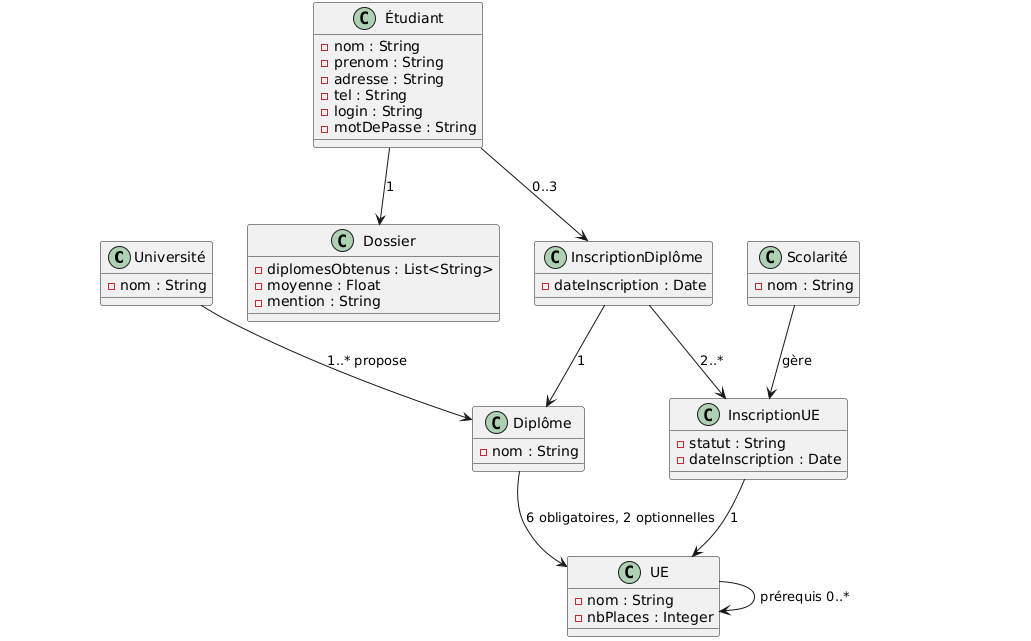
\includegraphics[width=\textwidth]{exo4.png}
  \caption{Diagramme de classes pour l'exercice 4}
\end{figure}

\section*{Exercice 5}

\begin{figure}[H]
  \centering
  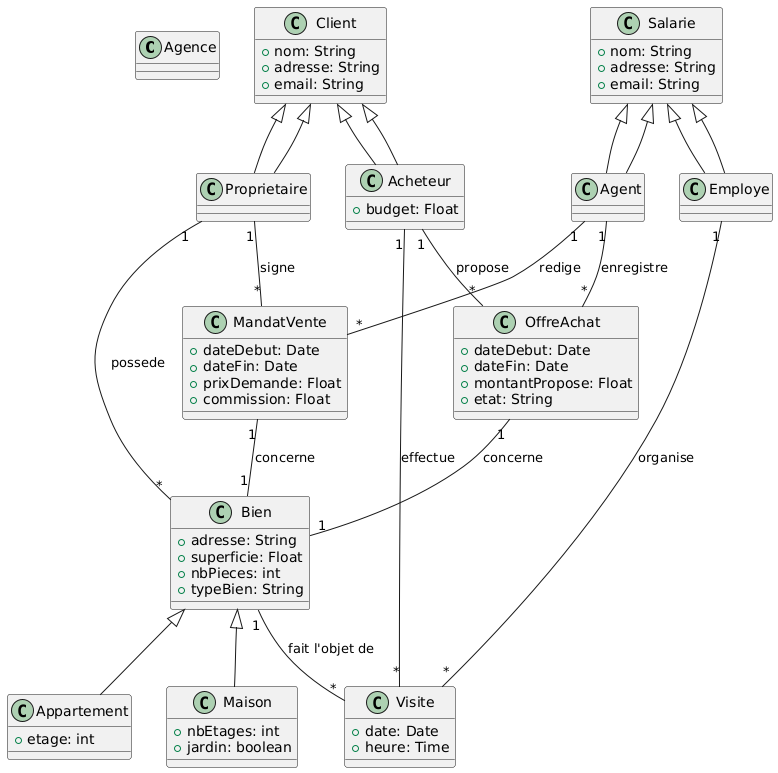
\includegraphics[width=\textwidth]{exo5.png}
  \caption{Diagramme de classes pour l'exercice 5}
\end{figure}

\end{document}